\documentclass{article}
\usepackage{graphicx}
\usepackage[utf8]{inputenc}
\usepackage[T1]{fontenc}
\usepackage{fouriernc}
\usepackage[margin=1in]{geometry}
\usepackage{amsmath}
\begin{document}

\begin{titlepage}
	\centering 
	\scshape
	\vspace*{\baselineskip}
	\rule{\textwidth}{1.6pt}\vspace*{-\baselineskip}\vspace*{2pt}
	\rule{\textwidth}{0.4pt} 
	\vspace{0.75\baselineskip}
	
	{\Large CS 374 : Computational and Numerical Methods \\\vspace{0.75\baselineskip} Set 5}
	\vspace{0.75\baselineskip}
	
	\rule{\textwidth}{0.4pt}\vspace*{-\baselineskip}\vspace{3.2pt} 
	\rule{\textwidth}{1.6pt}
	
	\vspace{2\baselineskip}  
	The Bisection Method
	
	\vspace*{3\baselineskip}
	
	\vspace{0.5\baselineskip} %originally 0.5
	
	{\scshape\large Purvil Mehta (201701073) \\ Bhargey Mehta (201701074) \\} 
	
	\vspace{1\baselineskip} 
	
	\textit{Dhirubhai Ambani Institute of Information and Communication Technology \\ Gandhinagar\\} 
	\vspace*{2\baselineskip}
	\today


\end{titlepage}

\newpage
\tableofcontents
\newpage

\section{$f(x)$ = $x^6 - x - 1$}
\subsection{Plots}
\begin{figure}[!h]
    \centering
    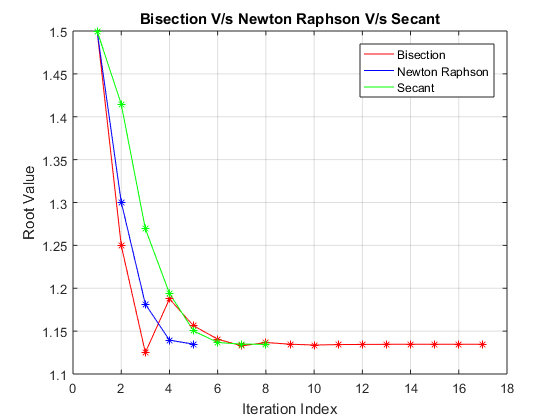
\includegraphics[scale=0.85]{1_1.png}
    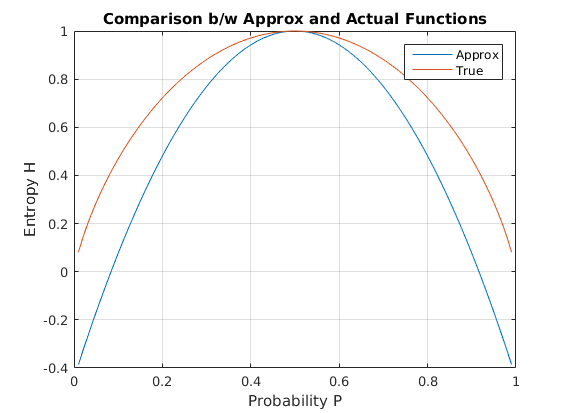
\includegraphics[scale=0.85]{1_2.png}
    \caption{Fig 1.1: Positive root of $x^6 - x -1 = 0$ 
     || Fig 1.2: Negative root of $x^6 - x -1 = 0$}
\end{figure}
\subsection{Tables}
\begin{table}[!h]
\centering{\Large
\begin{tabular}{|c|c|c|c|c|c|c|c|}\hline
ItrNo & $x_n$ & $f(x_n)$ & $f(x_n) - f(x_{n-1})$ &$x_n-x_{n-1}$ & $x_{n+1}$& $x_{n+1}-x_{n}$ \\ \hline
1 & 2      & 61      & 0        & 0        & 1.5    & 0        \\
2 & 1.5    & 8.8906  & -0.5     & -52.109  & 1.4147 & -0.08531 \\
3 & 1.4147 & 5.6016  & -0.08531 & -3.289   & 1.2694 & -0.14529 \\
4 & 1.2694 & 1.9147  & -0.14529 & -3.6869  & 1.194  & -0.07545 \\
5 & 1.194  & 0.70289 & -0.07545 & -1.2118  & 1.1502 & -0.04376 \\
6 & 1.1502 & 0.16516 & -0.04376 & -0.53774 & 1.1367 & -0.01344 \\
7 & 1.1367 & 0.02092 & -0.01344 & -0.14424 & 1.1348 & -0.00195 \\
8 & 1.1348 & 0.00076 & -0.00195 & -0.02016 & 1.1347 & -7e-05   \\
9 & 1.1347 & 0       & -7e-05   & -0.00076 & 1.1347 & 0        \\
\hline
\end{tabular}}
\caption{Positive Root of $x^6 - x - 1 =0$}
\end{table}

\begin{table}[!h]
\centering{\Large
\begin{tabular}{|c|c|c|c|c|c|c|c|}\hline
ItrNo & $x_n$ & $f(x_n)$ & $f(x_n) - f(x_{n-1})$ &$x_n-x_{n-1}$ & $x_{n+1}$& $x_{n+1}-x_{n}$ \\ \hline
1 & -1       & 1       & 0        & 0        & -1.5     & 0        \\
2 & -1.5     & 11.891  & -0.5     & 10.891   & -0.95409 & 0.54591  \\
3 & -0.95409 & 0.70837 & 0.54591  & -11.182  & -0.91951 & 0.03458  \\
4 & -0.91951 & 0.52391 & 0.03458  & -0.18446 & -0.82128 & 0.09822  \\
5 & -0.82128 & 0.12815 & 0.09822  & -0.39576 & -0.78948 & 0.03181  \\
6 & -0.78948 & 0.0316  & 0.03181  & -0.09656 & -0.77907 & 0.01041  \\
7 & -0.77907 & 0.00266 & 0.01041  & -0.02894 & -0.77811 & 0.00096  \\
8 & -0.77811 & 6e-05   & 0.00096  & -0.0026  & -0.77809 & 2e-05    \\
9 & -0.77809 & 0       & 2e-05    & -6e-05   & -0.77809 & 0        \\
\hline
\end{tabular}}
\caption{Negative Root of $x^6 - x - 1 =0$}
\end{table}

\newpage
\section{$f(x)$ = $x^3 - x^2 - x - 1$}
\subsection{Plots}
\begin{figure}[!h]
    \centering
    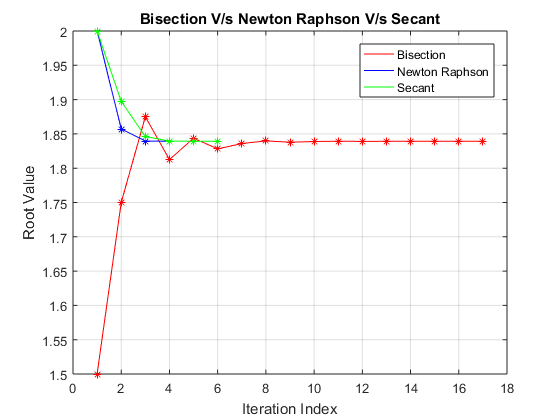
\includegraphics[scale=0.85]{2.png}
    \caption{Positive root of $x^3 - x^2 -x-1 = 0$}
\end{figure}
\subsection{Tables}
\begin{table}[!h]
\centering{\Large
\begin{tabular}{|c|c|c|c|c|c|c|c|}\hline
ItrNo & $x_n$ & $f(x_n)$ & $f(x_n) - f(x_{n-1})$ &$x_n-x_{n-1}$ & $x_{n+1}$& $x_{n+1}-x_{n}$ \\ \hline
1 & 2.5    & 5.875   & 0        & 0        & 2      & 0        \\
2 & 2      & 1       & -0.5     & -4.875   & 1.8974 & -0.10256 \\
3 & 1.8974 & 0.33357 & -0.10256 & -0.66643 & 1.8461 & -0.05134 \\
4 & 1.8461 & 0.03748 & -0.05134 & -0.29609 & 1.8396 & -0.0065  \\
5 & 1.8396 & 0.00172 & -0.0065  & -0.03576 & 1.8393 & -0.00031 \\
6 & 1.8393 & 1e-05   & -0.00031 & -0.00171 & 1.8393 & 0        \\
7 & 1.8393 & 0       & 0        & -1e-05   & 1.8393 & 0        \\
\hline
\end{tabular}}
\caption{Positive Root of $x^3 - x^2 - x - 1 =0$}
\end{table}

\newpage
\section{$f(x) = 1 +0.3cos(x) - x$}
\subsection{Plots}
\begin{figure}[!h]
    \centering
    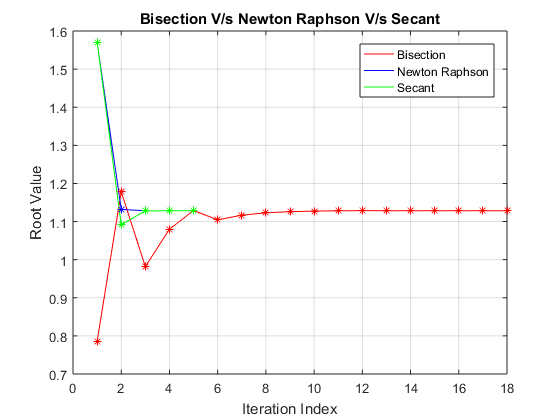
\includegraphics[scale=0.85]{3.png}
    \caption{Fig 1.1,1.2 : Positive root of $f(x) = 1 +0.3cos(x) - x$}
    \label{fig:ques3}
\end{figure}
\subsection{Tables}
\begin{table}[!h]
\centering{\Large
\begin{tabular}{|c|c|c|c|c|c|c|c|}\hline
ItrNo & $x_n$ & $f(x_n)$ & $f(x_n) - f(x_{n-1})$ &$x_n-x_{n-1}$ & $x_{n+1}$& $x_{n+1}-x_{n}$ \\ \hline
1 & 3.1416 & -2.4416 & 0        & 0        & 1.5708 & 0        \\
2 & 1.5708 & -0.5708 & -1.5708  & 1.8708   & 1.0915 & -0.47926 \\
3 & 1.0915 & 0.04681 & -0.47926 & 0.6176   & 1.1279 & 0.03632  \\
4 & 1.1279 & 0.00073 & 0.03632  & -0.04608 & 1.1284 & 0.00057  \\
5 & 1.1284 & 0       & 0.00057  & -0.00073 & 1.1284 & 0        \\
6 & 1.1284 & 0       & 0        & 0        & 1.1284 & 0        \\
\hline
\end{tabular}}
\caption{Positive Root of $f(x) = 1 +0.3cos(x) - x$}
\end{table}
\newpage



\section{$f(x) = 0.5 + \sin{x} - \cos{x}$}
\subsection{Plots}
\begin{figure}[!h]
    \centering
    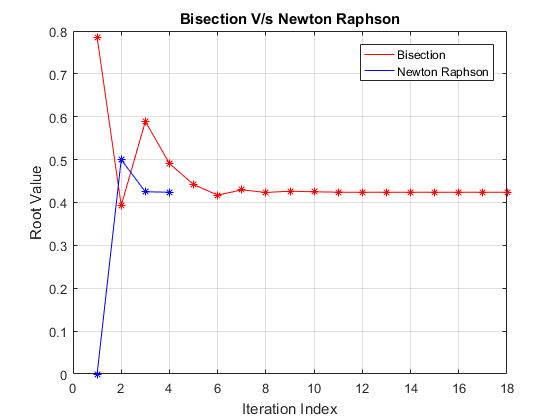
\includegraphics[scale=0.85]{4.png}
    \caption{Fig 1.1,1.2 : Positive root of $f(x) = 0.5 + \sin{x} - \cos{x}$}
\end{figure}
\subsection{Tables}
\begin{table}[!h]
\centering{\Large
\begin{tabular}{|c|c|c|c|c|c|c|c|}\hline
ItrNo & $x_n$ & $f(x_n)$ & $f(x_n) - f(x_{n-1})$ &$x_n-x_{n-1}$ & $x_{n+1}$& $x_{n+1}-x_{n}$ \\ \hline
1 & 1       & 0.80117 & 0        & 0        & 0.5     & 0        \\
2 & 0.5     & 0.10184 & -0.5     & -0.69933 & 0.42718 & -0.07282 \\
3 & 0.42718 & 0.00417 & -0.07282 & -0.09767 & 0.42407 & -0.00311 \\
4 & 0.42407 & 5e-05   & -0.00311 & -0.00412 & 0.42403 & -4e-05   \\
5 & 0.42403 & 0       & -4e-05   & -5e-05   & 0.42403 & 0        \\
\hline
\end{tabular}}
\caption{The smallest Positive Root of $f(x) = 0.5 + \sin{x} - \cos{x}$}
\end{table}
\newpage



\section{$f(x) = x - e^{-x}$}
\subsection{Plots}
\begin{figure}[!h]
    \centering
    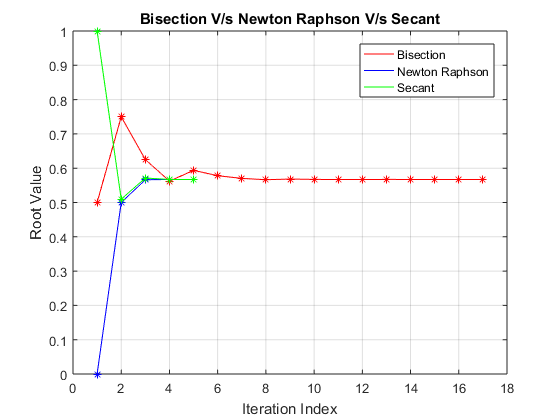
\includegraphics[scale=0.85]{5.png}
    \caption{Positive root of $f(x) = x - - e^{-x}$}
\end{figure}
\subsection{Tables}
\begin{table}[!h]
\centering{\Large
\begin{tabular}{|c|c|c|c|c|c|c|c|}\hline
ItrNo & $x_n$ & $f(x_n)$ & $f(x_n) - f(x_{n-1})$ &$x_n-x_{n-1}$ & $x_{n+1}$& $x_{n+1}-x_{n}$ \\ \hline
1 & 1.5     & -1.2769  & 0        & 0        & 1       & 0        \\
2 & 1       & -0.63212 & -0.5     & 0.64475  & 0.50979 & -0.49021 \\
3 & 0.50979 & 0.09083  & -0.49021 & 0.72295  & 0.57138 & 0.06159  \\
4 & 0.57138 & -0.00663 & 0.06159  & -0.09746 & 0.56719 & -0.00419 \\
5 & 0.56719 & -7e-05   & -0.00419 & 0.00656  & 0.56714 & -4e-05   \\
6 & 0.56714 & 0        & -4e-05   & 7e-05    & 0.56714 & 0        \\
\hline
\end{tabular}}
\caption{The smallest Positive Root of $f(x) = x - e^{-x}$}
\end{table}
\newpage


\section{$f(x) = \sin{x} - e^{-x}$}
\subsection{Plots}
\begin{figure}[!h]
    \centering
    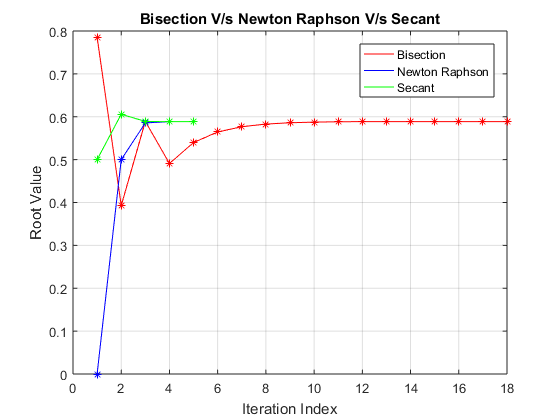
\includegraphics[scale=0.85]{6_1.png}
    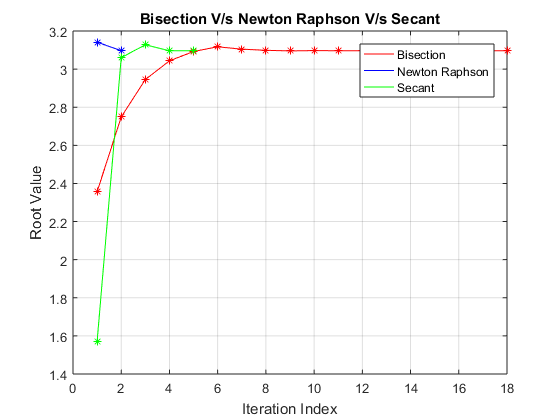
\includegraphics[scale=0.85]{6_2.png}
    \caption{1.1 : First smallest Positive root of $f(x) = \sin{x} - e^{-x}$ 
     || 1.2 : Second Smallest Positive root of $f(x) = \sin{x} - e^{-x}$}
\end{figure}

\subsection{Tables}
\begin{table}[!h]
\centering{\Large
\begin{tabular}{|c|c|c|c|c|c|c|c|}\hline
ItrNo & $x_n$ & $f(x_n)$ & $f(x_n) - f(x_{n-1})$ &$x_n-x_{n-1}$ & $x_{n+1}$& $x_{n+1}-x_{n}$ \\ \hline
1 & 1       & -0.47359 & 0        & 0        & 0.5     & 0        \\
2 & 0.5     & 0.12711  & -0.5     & 0.6007   & 0.6058  & 0.1058   \\
3 & 0.6058  & -0.02378 & 0.1058   & -0.15088 & 0.58912 & -0.01667 \\
4 & 0.58912 & -0.00082 & -0.01667 & 0.02296  & 0.58853 & -0.0006  \\
5 & 0.58853 & 1e-05    & -0.0006  & 0.00083  & 0.58853 & 0        \\
6 & 0.58853 & 0        & 0        & -1e-05   & 0.58853 & 0        \\
\hline
\end{tabular}}
\caption{The first smallest Positive Root of $f(x) = \sin{x} - e^{-x}$}
\end{table}
\begin{table}[!h]
\centering{\Large
\begin{tabular}{|c|c|c|c|c|c|c|c|}\hline
ItrNo & $x_n$ & $f(x_n)$ & $f(x_n) - f(x_{n-1})$ &$x_n-x_{n-1}$ & $x_{n+1}$& $x_{n+1}-x_{n}$ \\ \hline
1 & 3.1416 & 0.04321  & 0        & 0        & 1.5708 & 0        \\
2 & 1.5708 & -0.79212 & -1.5708  & -0.83533 & 3.0603 & 1.4895   \\
3 & 3.0603 & -0.0343  & 1.4895   & 0.75782  & 3.1277 & 0.06742  \\
4 & 3.1277 & 0.02997  & 0.06742  & 0.06427  & 3.0963 & -0.03144 \\
5 & 3.0963 & -5e-05   & -0.03144 & -0.03003 & 3.0964 & 5e-05    \\
6 & 3.0964 & 0        & 5e-05    & 5e-05    & 3.0964 & 0        \\
\hline
\end{tabular}}
\caption{The Second smallest Positive Root of $f(x) = \sin{x} - e^{-x}$}
\end{table}
\newpage




\section{$f(x) = x^3 -2x -2$}
\subsection{Plots}
\begin{figure}[!h]
    \centering
    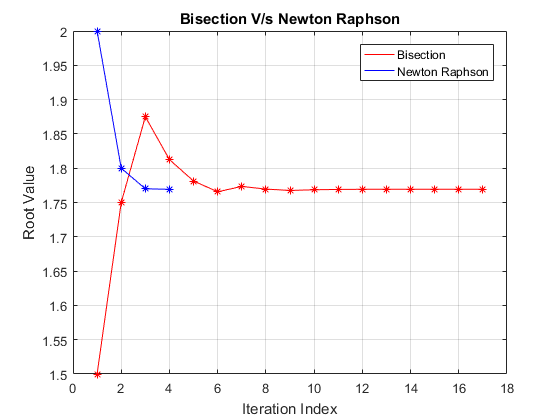
\includegraphics[scale=0.85]{7.png}
    \caption{Positive root of $f(x) = x^3 -2x -2$ }
\end{figure}
\subsection{Tables}
\begin{table}[!h]
\centering{\Large
\begin{tabular}{|c|c|c|c|c|c|c|c|}\hline
ItrNo & $x_n$ & $f(x_n)$ & $f(x_n) - f(x_{n-1})$ &$x_n-x_{n-1}$ & $x_{n+1}$& $x_{n+1}-x_{n}$ \\ \hline
1 & 2.5    & 8.625   & 0        & 0        & 2      & 0        \\
2 & 2      & 2       & -0.5     & -6.625   & 1.8491 & -0.15094 \\
3 & 1.8491 & 0.62383 & -0.15094 & -1.3762  & 1.7806 & -0.06842 \\
4 & 1.7806 & 0.0845  & -0.06842 & -0.53933 & 1.7699 & -0.01072 \\
5 & 1.7699 & 0.00458 & -0.01072 & -0.07992 & 1.7693 & -0.00061 \\
6 & 1.7693 & 4e-05   & -0.00061 & -0.00454 & 1.7693 & -1e-05   \\
7 & 1.7693 & 0       & -1e-05   & -4e-05   & 1.7693 & 0   \\
\hline
\end{tabular}}
\caption{The Positive Root of $f(x) = x^3 -2x -2$}
\end{table}



\newpage
\section{$f(x) = x^4 -x -1$}
\subsection{Plots}
\begin{figure}[!h]
    \centering
    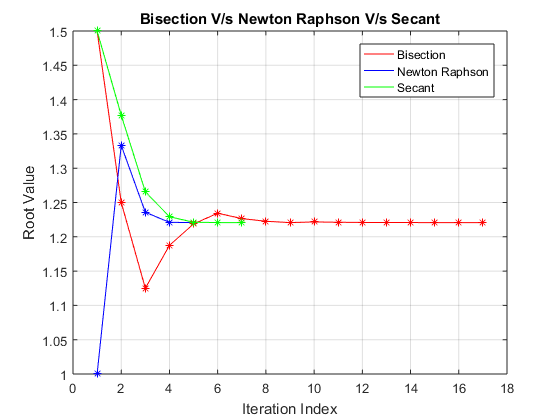
\includegraphics[scale=0.85]{8_1.png}
    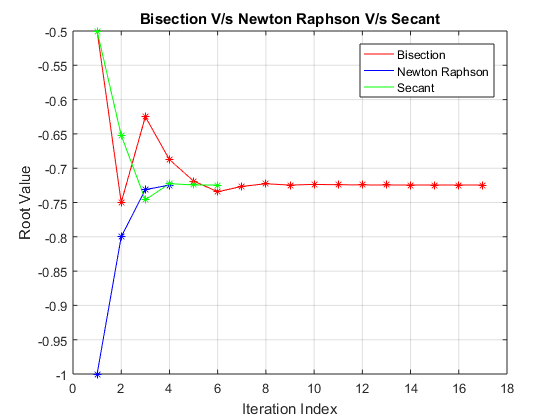
\includegraphics[scale=0.85]{8_2.png}
    \caption{1.1 : Positive root of $f(x) = x^4 -x -1$ | 1.2 : Negative Root of $f(x) = x^4 - x -1$}
    \label{fig:ques8}
\end{figure}
\subsection{Tables}
\begin{table}[!h]
\centering{\Large
\begin{tabular}{|c|c|c|c|c|c|c|c|}\hline
ItrNo & $x_n$ & $f(x_n)$ & $f(x_n) - f(x_{n-1})$ &$x_n-x_{n-1}$ & $x_{n+1}$& $x_{n+1}-x_{n}$ \\ \hline
1 & 2      & 13      & 0        & 0        & 1.5    & 0        \\
2 & 1.5    & 2.5625  & -0.5     & -10.438  & 1.3773 & -0.12275 \\
3 & 1.3773 & 1.2206  & -0.12275 & -1.3419  & 1.2656 & -0.11166 \\
4 & 1.2656 & 0.29986 & -0.11166 & -0.92076 & 1.2292 & -0.03636 \\
5 & 1.2292 & 0.05384 & -0.03636 & -0.24603 & 1.2213 & -0.00796 \\
6 & 1.2213 & 0.00325 & -0.00796 & -0.05059 & 1.2208 & -0.00051 \\
7 & 1.2208 & 4e-05   & -0.00051 & -0.00321 & 1.2207 & -1e-05   \\
8 & 1.2207 & 0       & -1e-05   & -4e-05   & 1.2207 & 0\\
\hline
\end{tabular}}
\caption{The Positive Root of $f(x) = x^4 -x -1$}
\end{table}
\begin{table}[!h]
\centering{\Large
\begin{tabular}{|c|c|c|c|c|c|c|c|}\hline
ItrNo & $x_n$ & $f(x_n)$ & $f(x_n) - f(x_{n-1})$ &$x_n-x_{n-1}$ & $x_{n+1}$& $x_{n+1}-x_{n}$ \\ \hline
1 & -1       & 1        & 0        & 0        & -0.5     & 0        \\
2 & -0.5     & -0.4375  & 0.5      & -1.4375  & -0.65217 & -0.15217 \\
3 & -0.65217 & -0.16692 & -0.15217 & 0.27058  & -0.74605 & -0.09388 \\
4 & -0.74605 & 0.05584  & -0.09388 & 0.22276  & -0.72252 & 0.02353  \\
5 & -0.72252 & -0.00497 & 0.02353  & -0.06081 & -0.72444 & -0.00192 \\
6 & -0.72444 & -0.00013 & -0.00192 & 0.00483  & -0.72449 & -5e-05   \\
7 & -0.72449 & 0        & -5e-05   & 0.00013  & -0.72449 & 0        \\
\hline
\end{tabular}}
\caption{The Negative Root of $f(x) = x^4 -x -1$}
\end{table}



\newpage
\section{$f(x) = e^x -x -2$}
\subsection{Plots}
\begin{figure}[!h]
    \centering
    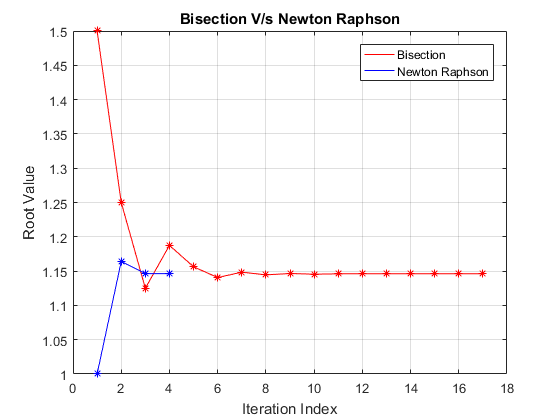
\includegraphics[scale=0.85]{9.png}
    \caption{Positive root of $f(x) = e^x -x -2$ }
\end{figure}
\subsection{Tables}
\begin{table}[!h]
\centering{\Large
\begin{tabular}{|c|c|c|c|c|c|c|c|}\hline
ItrNo & $x_n$ & $f(x_n)$ & $f(x_n) - f(x_{n-1})$ &$x_n-x_{n-1}$ & $x_{n+1}$& $x_{n+1}-x_{n}$ \\ \hline
1 & 1.5    & 0.98169  & 0        & 0        & 1      & 0        \\
2 & 1      & -0.28172 & -0.5     & -1.2634  & 1.1115 & 0.11149  \\
3 & 1.1115 & -0.0726  & 0.11149  & 0.20911  & 1.1502 & 0.03871  \\
4 & 1.1502 & 0.00863  & 0.03871  & 0.08123  & 1.1461 & -0.00411 \\
5 & 1.1461 & -0.00022 & -0.00411 & -0.00885 & 1.1462 & 0.0001   \\
6 & 1.1462 & 0        & 0.0001   & 0.00022  & 1.1462 & 0        \\
\hline
\end{tabular}}
\caption{The Positive Root of $f(x) = e^x -x -2$}
\end{table}



\newpage
\section{$f(x) = 1 -x +\sin{x}$}
\subsection{Plots}
\begin{figure}[!h]
    \centering
    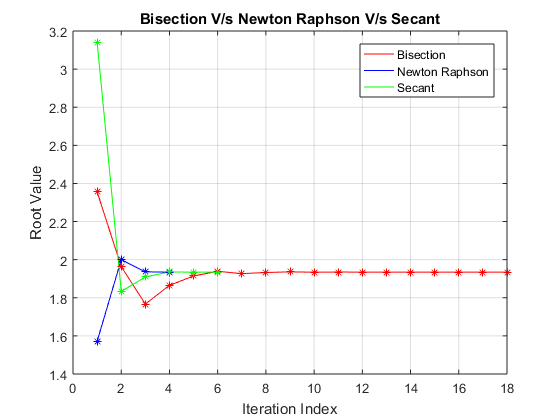
\includegraphics[scale=0.85]{10.png}
    \caption{Smallest Positive root of $f(x) = 1 -x +\sin{x}$ }
\end{figure}
\subsection{Tables}
\begin{table}[!h]
\centering{\Large
\begin{tabular}{|c|c|c|c|c|c|c|c|}\hline
ItrNo & $x_n$ & $f(x_n)$ & $f(x_n) - f(x_{n-1})$ &$x_n-x_{n-1}$ & $x_{n+1}$& $x_{n+1}-x_{n}$ \\ \hline
1 & 1.5708 & 0.4292   & 0        & 0        & 3.1416 & 0        \\
2 & 3.1416 & -2.1416  & 1.5708   & -2.5708  & 1.8331 & -1.3086  \\
3 & 1.8331 & 0.13276  & -1.3086  & 2.2744   & 1.9094 & 0.07638  \\
4 & 1.9094 & 0.03378  & 0.07638  & -0.09898 & 1.9355 & 0.02607  \\
5 & 1.9355 & -0.00127 & 0.02607  & -0.03504 & 1.9346 & -0.00094 \\
6 & 1.9346 & 1e-05    & -0.00094 & 0.00128  & 1.9346 & 1e-05    \\
7 & 1.9346 & 0        & 1e-05    & -1e-05   & 1.9346 & 0        \\
\hline
\end{tabular}}
\caption{The smallest Positive Root of $f(x) = 1 -x +\sin{x}$}
\end{table}



\newpage
\section{$f(x) = -x +\tan{x}$} 
\subsection{Plots}
\begin{figure}[!h]
    \centering
    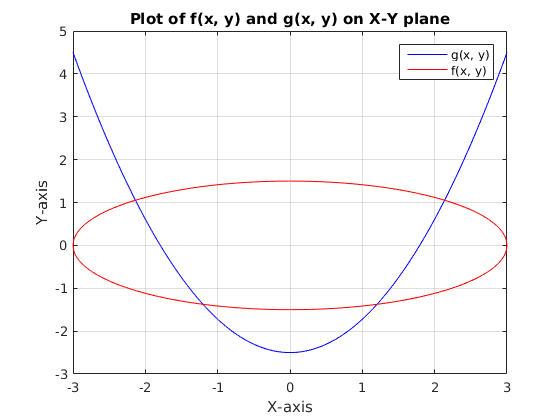
\includegraphics[scale=0.85]{11_1.png}
    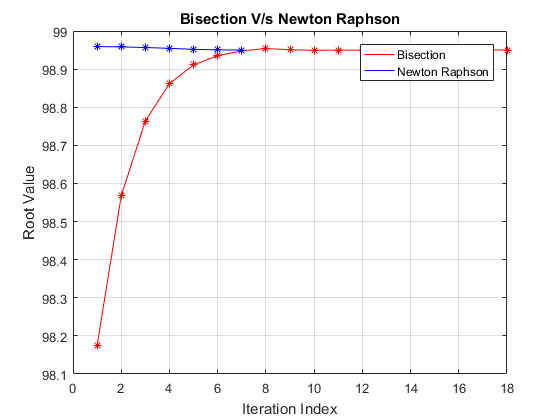
\includegraphics[scale=0.85]{11_2.png}
    \caption{1.1 : First Root of $f(x) = -x +\tan{x}$ | 1.2 :  Root of $f(x) = -x + \tan{x}$ near $x = 100$}
\end{figure}


\begin{table}[!ht]
\centering{\Large
\begin{tabular}{|c|c|c|c|c|c|c|c|}\hline
ItrNo & $x_n$ & $f(x_n)$ & $f(x_n) - f(x_{n-1})$ &$x_n-x_{n-1}$ & $x_{n+1}$& $x_{n+1}-x_{n}$ \\ \hline
1 & 4.7024 & 95.294  & 0        & 0        & 4.6124 & 0        \\
2 & 4.6124 & 5.3543  & -0.09    & -89.94   & 4.607  & -0.00536 \\
3 & 4.607  & 4.8493  & -0.00536 & -0.50497 & 4.5556 & -0.05145 \\
4 & 4.5556 & 1.7692  & -0.05145 & -3.0801  & 4.526  & -0.02955 \\
5 & 4.526  & 0.77754 & -0.02955 & -0.99167 & 4.5028 & -0.02317 \\
6 & 4.5028 & 0.19952 & -0.02317 & -0.57803 & 4.4948 & -0.008   \\
7 & 4.4948 & 0.02935 & -0.008   & -0.17017 & 4.4935 & -0.00138 \\
8 & 4.4935 & 0.0013  & -0.00138 & -0.02805 & 4.4934 & -6e-05   \\
9 & 4.4934 & 1e-05   & -6e-05   & -0.00129 & 4.4934 & 0 \\
\hline
\end{tabular}}
\caption{The smallest Positive Root of $f(x) = -x +\tan{x}$}
\end{table}
\begin{table}[!ht]
\centering{\Large
\begin{tabular}{|c|c|c|c|c|c|c|c|}\hline
ItrNo & $x_n$ & $f(x_n)$ & $f(x_n) - f(x_{n-1})$ &$x_n-x_{n-1}$ & $x_{n+1}$& $x_{n+1}-x_{n}$ \\ \hline
1 & 98.95  & 1.0465   & 0        & 0        & 98.86  & 0        \\
2 & 98.86  & -88.894  & -0.09    & -89.94   & 98.949 & 0.08895  \\
3 & 98.949 & -8.4321  & 0.08895  & 80.461   & 98.958 & 0.00932  \\
4 & 98.958 & 480.67   & 0.00932  & 489.11   & 98.949 & -0.00916 \\
5 & 98.949 & -7.0959  & -0.00916 & -487.77  & 98.949 & 0.00013  \\
6 & 98.949 & -5.9575  & 0.00013  & 1.1384   & 98.95  & 0.0007   \\
7 & 98.95  & 0.49221  & 0.0007   & 6.4497   & 98.95  & -5e-05   \\
8 & 98.95  & -0.03137 & -5e-05   & -0.52358 & 98.95  & 0        \\
9 & 98.95  & -0.00016 & 0        & 0.03122  & 98.95  & 0       \\
\hline
\end{tabular}}
\caption{The Positive Root of $f(x) = -x +\tan{x}$ around 100}
\end{table}
\end{document}